\documentclass{beamer}
\usepackage{pst-plot}
\usepackage[utf8]{inputenc}
\usepackage{pgf,pgfplots}
\usepackage{graphicx}
\usepackage[english,russian]{babel}
\usepackage{ragged2e}
\renewcommand{\raggedright}{\leftskip=0pt \rightskip=0pt plus 0cm}
\setbeamertemplate{caption}[numbered]
\setbeamertemplate{navigation symbols}{}
% Стиль презентации
\usetheme{Warsaw}
\begin{document}
	\title{Отчет о выполнении  II задания по практикуму}  
	\author{Капитанов Филипп, Ширяев Павел, Сабурова Анна, Мешина Злата}
	\institute{Московский государственный университет им. Ломоносова}
	\date{Москва, 2018} 
	% Создание заглавной страницы
	\frame{\titlepage} 
	% Автоматическая генерация содержания
	\frame{\frametitle{Постановка задачи}
		\begin{itemize}
			\item Есть два поставщика стали: {\bf Westeros Inc. и Harpy \& Co.} \\*Необходимо выбрать компанию, с которой следует заключить эксклюзивный договор на поставку стали.
			\item Необходимо провести {\bf разведывательный анализ данных} с целью ответа на вопрос: {\it "<С каким из поставщиков стали следует заключить договор?">}
		\end{itemize}\tableofcontents}
			
	\begin{frame}
		\frametitle{Исходные данные}
		\begin{itemize}
			\item Дан CSV-файл с данными о производстве оружия и количестве единиц сломанного оружия за каждый месяц каждым из кузнецов.
		\end{itemize}
	\end{frame}
	
	\begin{frame}
		\frametitle{Описание выполнения задания}
		\begin{itemize}
			\item<1-> Было рассмотрено несколько метрик, для сравнения качества продукции: 
			\begin{enumerate}
				\item Метрика показывает среднее число поломанной продукции после каждого месяца эксплуатации, т.е сколько мечей сломалось в среднем после одного месяца эксплуатации, сколько мечей сломалось после двух месяцев эксплеатации и т.д.
				\item Метрика показывает общий срок службы продукции по месяцам. Т.е. сколько суммарно прослужили мечи произведенные в первый месяц, во второй и т.д.
				\item Метрика показывает суммарное число сломанной продукции по месяцам. Т.е. сколько сломалось продукции после первого месяца службы, после второго и т.д.
			\end{enumerate}
		\end{itemize}
	\end{frame}
	\begin{frame}
		\frametitle{Описание выполнения задания}
		Для каждой метрики были построеные box plot и bar plot. Сравнивая данные графические отображения метрик, можно сделать выводы о качестве продукции.
		\\*
		Boxplot (ящик с усами или диаграмма размаха)
		График показывает сразу несколько параметров распределения:
		медиану - линия внутри ящика;
		стенками ящика (квартили 0.25 и 0.75) ограничены 50\% выборки;
		Длинна усов рассчитывается по-разомну.
		Это может быть просто минимальное и максимальное значения в выборке. Второй вариант - полторы ширины ящика (расстояния между квартилями 0.25 и 0.75). Тогда точками отмечаются выбросы. В нашей программе это просто минимальное и максимальное значения в выборке. 
	\end{frame}
	\begin{frame}[shrink=4]
		\frametitle{Описание выполнения задания}
		\framesubtitle{Метрика №1}
		\begin{figure}[h!]
			\begin{minipage}[h]{0.49\linewidth}
				\center{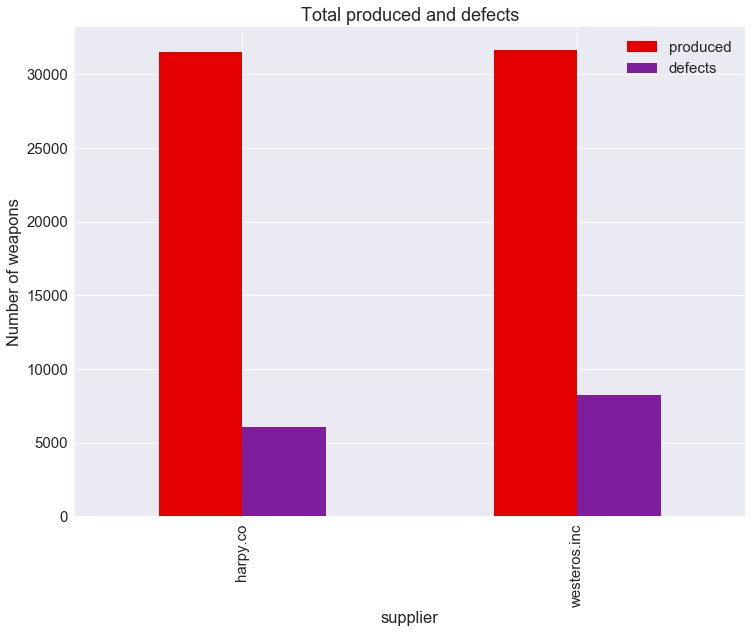
\includegraphics[width=1\linewidth]{1} \\ а) Bar plot}
			\end{minipage}
			\hfill
			\begin{minipage}[h]{0.49\linewidth}
				\center{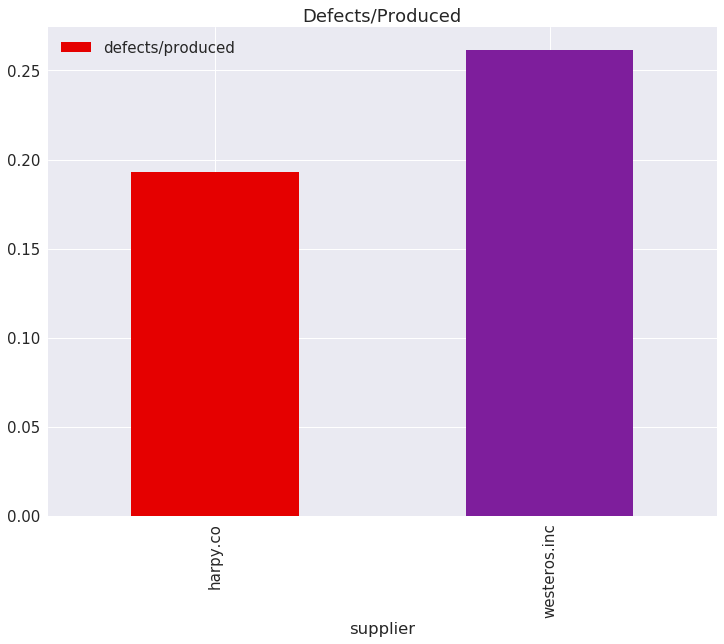
\includegraphics[width=1\linewidth]{2} \\ б) Box plot}
			\end{minipage}
			\caption{Среднее число дефектов в месяц}
			\label{ris:1}
		\end{figure}
		По первому графику сложно сделать какие-то выводы, т.к. в первые три месяца мечи из стали Harpy \& Co почти не ломаются, зато с 4 месяца количество сломанных мечей резко возрастает. А для мечей из стали Westeros Inc характерно, что ломается примерно одинаковое количество каждый месяц. Но при это медиана для компании Harpy \& Co ниже.
	\end{frame}
	\begin{frame}[shrink=4]
		\frametitle{Описание выполнения задания}
		\framesubtitle{Метрика №2}
		\begin{figure}[h!]
			\begin{minipage}[h]{0.49\linewidth}
				\center{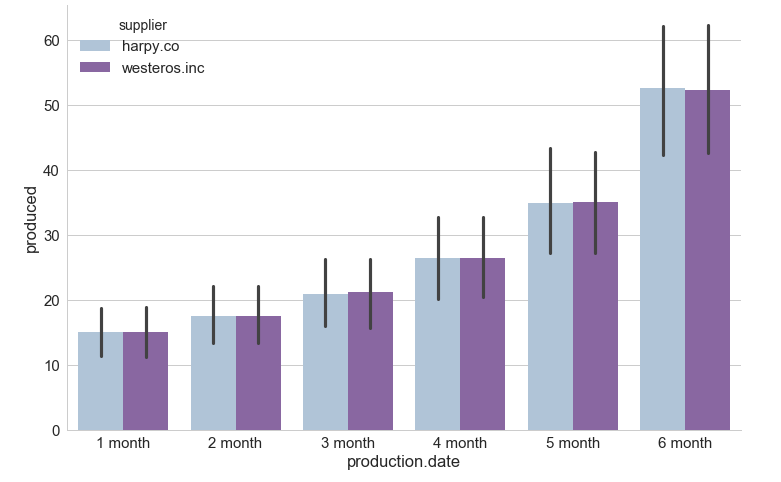
\includegraphics[width=1\linewidth]{3} \\ а) Bar plot}
			\end{minipage}
			\hfill
			\begin{minipage}[h]{0.49\linewidth}
				\center{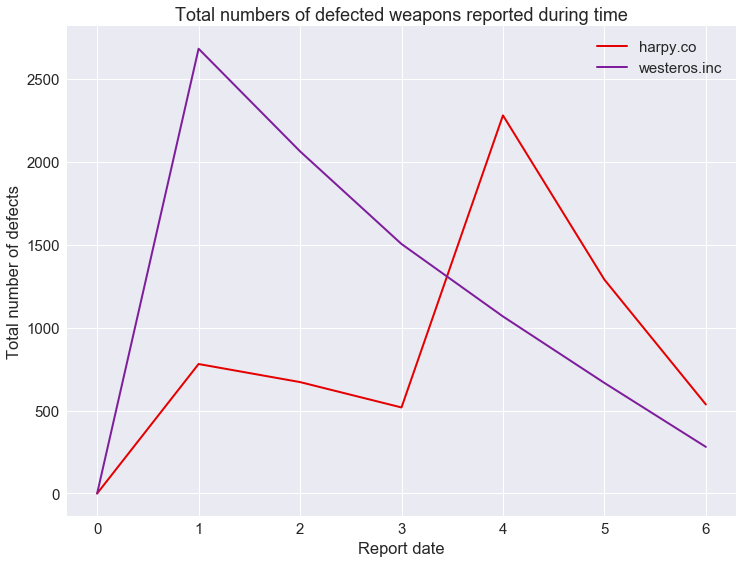
\includegraphics[width=1\linewidth]{4} \\ б) Box plot}
			\end{minipage}
			\caption{Суммарный срок службы}
			\label{ris:2}
		\end{figure}
		На данных графиках показан важный критерий, это общий срок службы мечей, но как видно из графиков данные параметры почти не отличаются по двум компаниям, результат немного лучше у компании Westeris Inc, это видно и из Bar plot и из  Box plot. 
	\end{frame}
	\begin{frame}[shrink=4]
		\frametitle{Описание выполнения задания}
		\framesubtitle{Метрика №3}
		\begin{figure}[h!]
			\begin{minipage}[h]{0.49\linewidth}
				\center{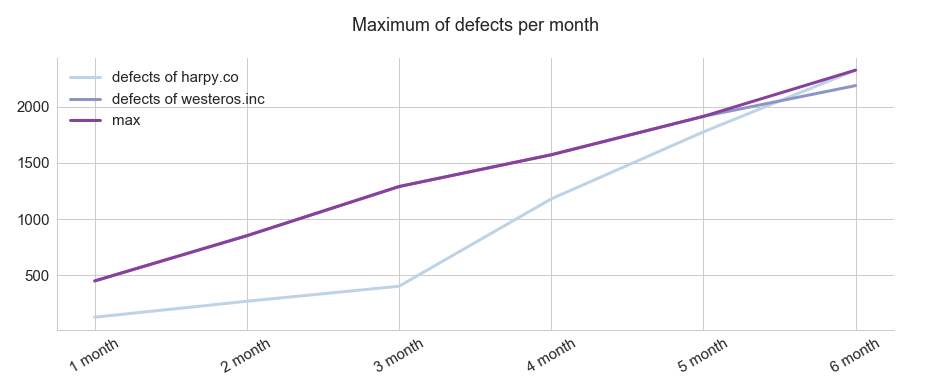
\includegraphics[width=1\linewidth]{5} \\ а) Bar plot}
			\end{minipage}
			\hfill
			\begin{minipage}[h]{0.49\linewidth}
				\center{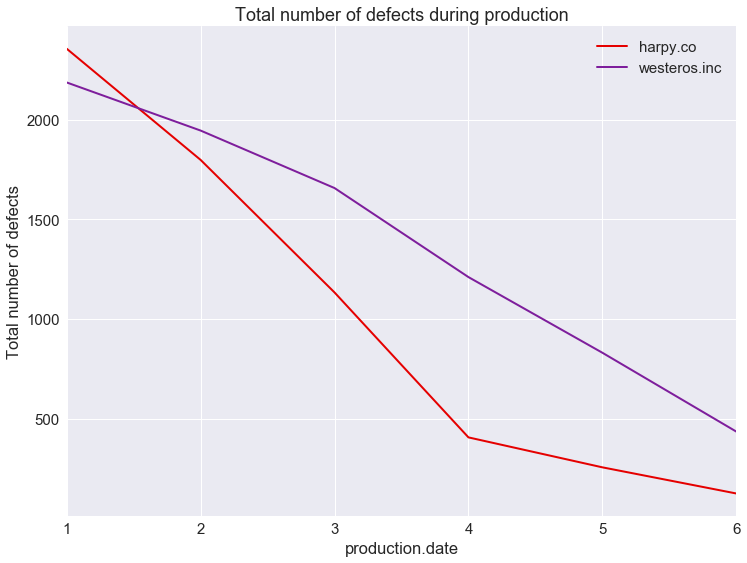
\includegraphics[width=1\linewidth]{6} \\ б) Box plot}
			\end{minipage}
			\caption{Общее число мечей без дефектов}
			\label{ris:3}
		\end{figure}
		На данном слайде представлен еще один важный показатель, это количество целых мечей. По данному показателю компания Harpy \& Co сильно опережает компанию Westeros Inc.
	\end{frame}
	\begin{frame}
	\frametitle{Анализ результатов}
		\begin{itemize}
			\item {Как было замечено выше, первая метрика не дает однозначной оценки при разведывательном анализе без использования дополнительных статистических методов.}
			\item {Вторая метрика весьма важна при оценке продукта, но у двух компаний результаты почти не различимы, поэтому по данному критерию сложно сделать выбор в пользу какой-либо компании. }
			\item {Третья метрика тоже показывает важный критерий, т.к. чем больше число целых мечей, тем большее число воинов могут участвовать в сражениях одновременно и тем выше численность войска. Численность войска является важным параметром при прочих равных условиях, особенно этот критерий важен для нападающей стороны.}
			\item {Можно сделать вывод, что предпочтительнее закупать сталь у компании Harpy \& Co.}
		\end{itemize}
	\end{frame}
	\begin{frame}
		\frametitle{Работу выполняли}
		\begin{itemize}
			\item Капитанов Филипп, Ширяев Павел, Сабурова Анна, Мешина Злата, студенты 3 курса ВМК МГУ, кафедры исследования операций, 312 группы. \\Все этапы работы (разработка алгоритма, написание программы, написание презентации)
		\end{itemize}	
	\end{frame}
\end{document}